The Schnakenberg equations, originally discussed in \cite{schnakenberg79}, is an example of pattern forming reactions that will be relevant to our models of \cref{ch:Bulk_surface_model,ch:Numerical_Analysis}. They are given by

\begin{equation}
    \label{eq:schnakenberg_reactions}
    f(u, v) = a - u + u^2 v \qquad \text{and} \qquad g(u,v) = b - u^2 v,
\end{equation}

\noindent
where $a$ and $b$ are positive real numbers representing constant production of both chemical species. In \cite{murray03}, a detailed analysis is given into the specific conditions for these reactions to form Turing patterns in one-dimensional domains. As a result, we get conditions for the parameters in the model that define a subset of the parameter space within which Turing instabilities take place, referred to as the \emph{Turing space}. For fixed $d$, this subset is given by the area between the two curves

\begin{align*}
    a &> \frac{1}{2} u_0 \left(1 - u_0^2\right), & b &= \frac{1}{2} u_0 \left(1 + u_0^2\right), \\
    a &< \frac{1}{2} u_0 \left(1 - \frac{2u_0}{\sqrt{d}} - \frac{u_0^2}{d}\right), & b &= \frac{1}{2} u_0 \left(1 + \frac{2u_0}{\sqrt{d}} + \frac{u_0^2}{d}\right),
\end{align*}

\noindent
parameterised by $u_0$, see \cref{fig:turingspace}. If $(a, b)$ is in between these two curves and $\gamma$ is high enough, a Turing instability will take place. You can see that the Turing space grows as larger values of $d$ are chosen. In \cref{fig:schnakenberg_frames_1-3,fig:schnakenberg_frames_4-6}, a simulation of this model is shown with parameters within the Turing space. In this simulation, the domain is $\Omega = (-8, 8)^2$ and the parameters are set to $d = 50$, $a = 0.1$, $b = 0.9$ and $\gamma = 8$. The initial conditions are set to

\begin{equation}\label{eq:schnakenberg_initial}
    u_0(x) = U + f(x) \qquad \text{and} \qquad v_0(x) = V + g(x),
\end{equation}

\noindent
where

\begin{equation}
    \label{eq:schnakenberg_steadystates}
    U := a + b \qquad \text{and} \qquad V := \frac{b}{(a + b)^2}
\end{equation}

\noindent
are the corresponding uniform steady states and $f$ and $g$ are independent noise functions whose values are uniformly sampled from $(-0.1, 0.1)$. \todo{Is this mixing the continuous problem and discretised simulation too much?}

\todo{What is the standard way of showing these simulations?}

\begin{figure}[!t]
    \centering
    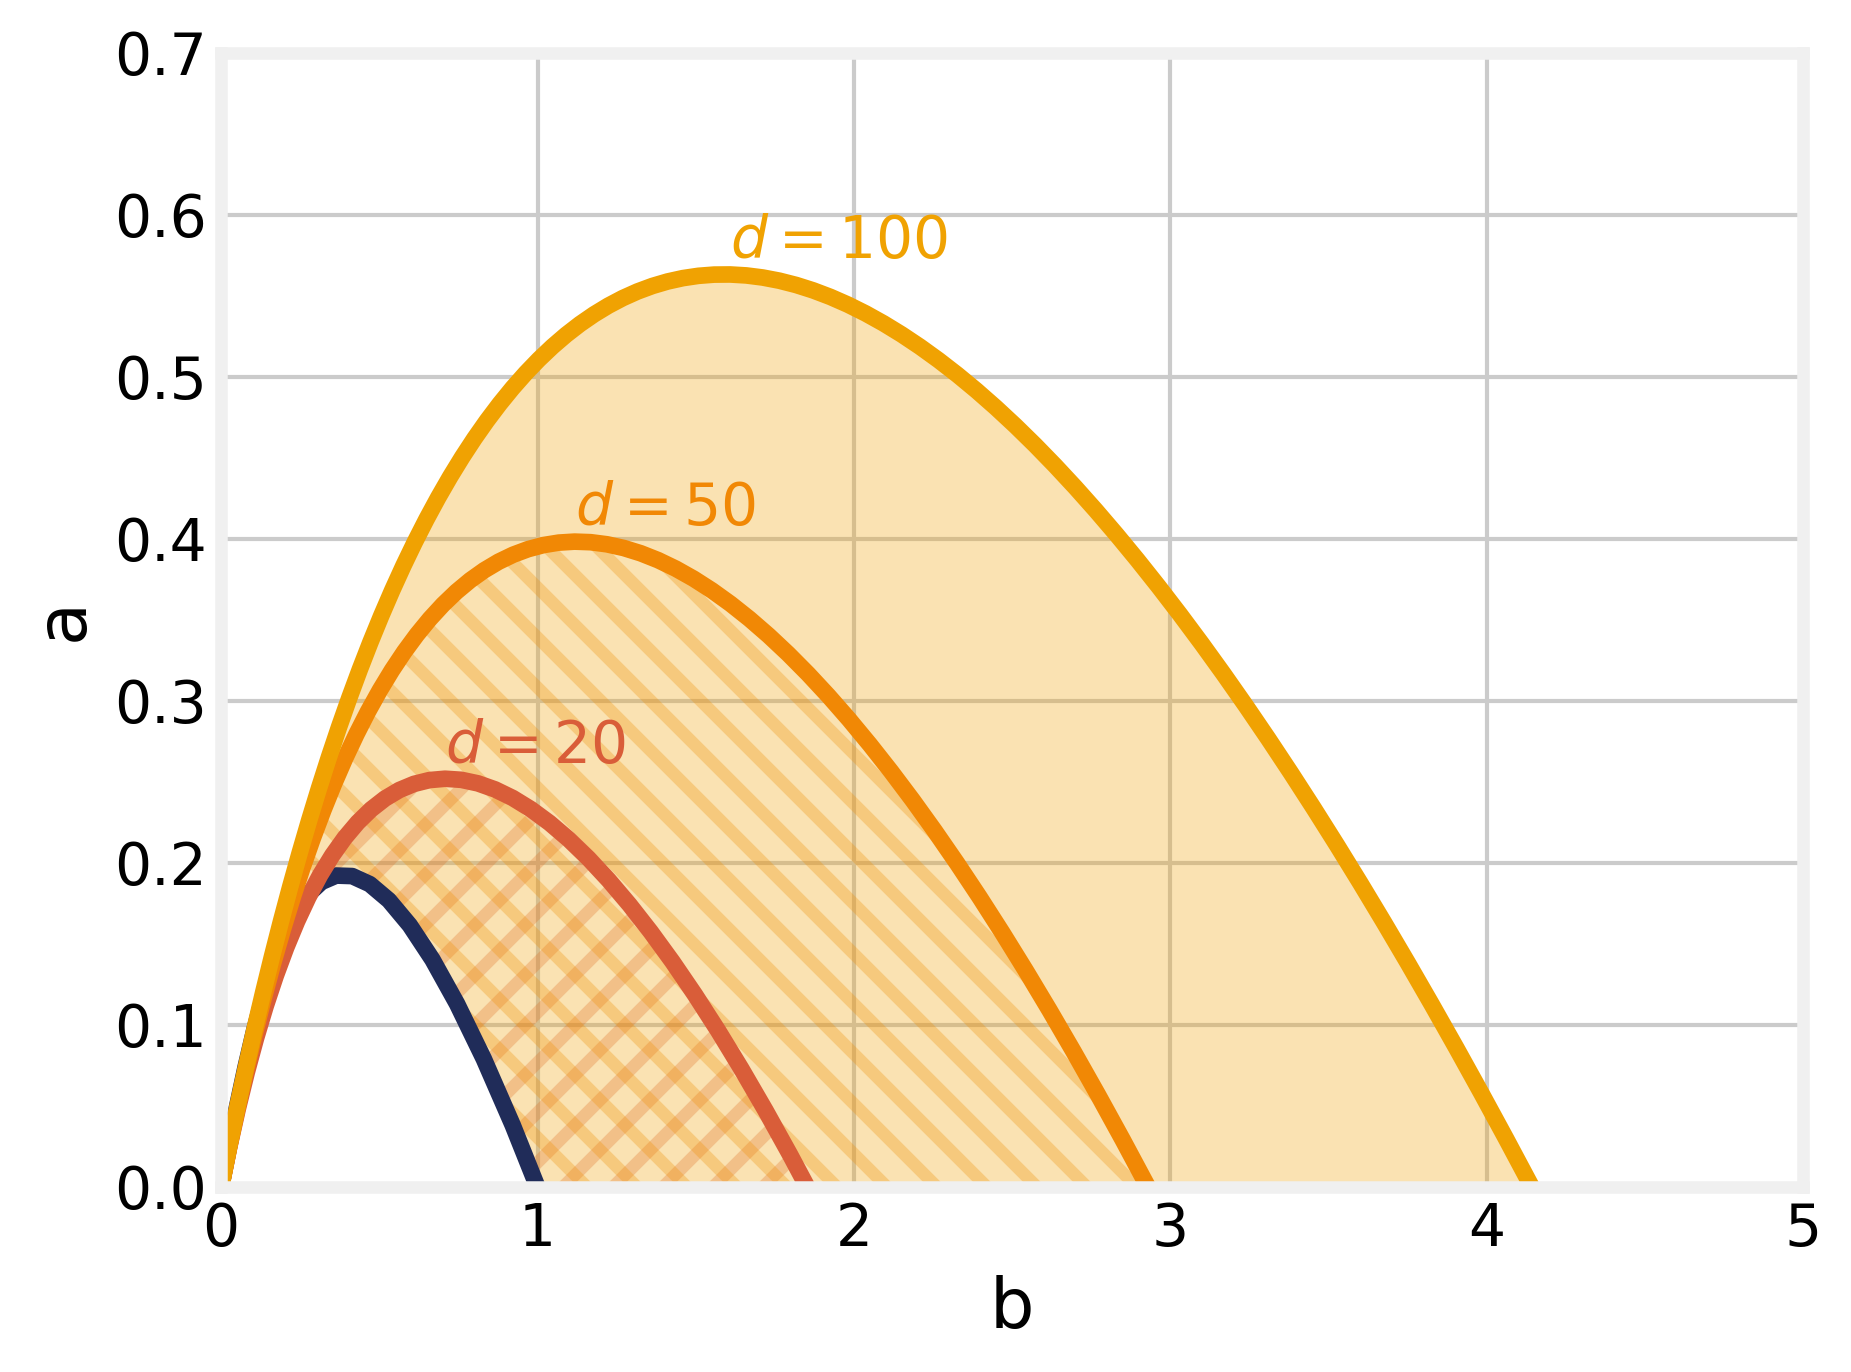
\includegraphics[width=0.5\linewidth]{img/Turing_space.png}
    \caption{The Turing space for \cref{eq:schnakenberg_reactions} plotted for $d = 20$, $d = 50$ and $d = 100$.}
    \label{fig:turingspace}
\end{figure}

\begin{figure}[htbp]
    \centering

    \begin{subfigure}{\textwidth}
        \centering
        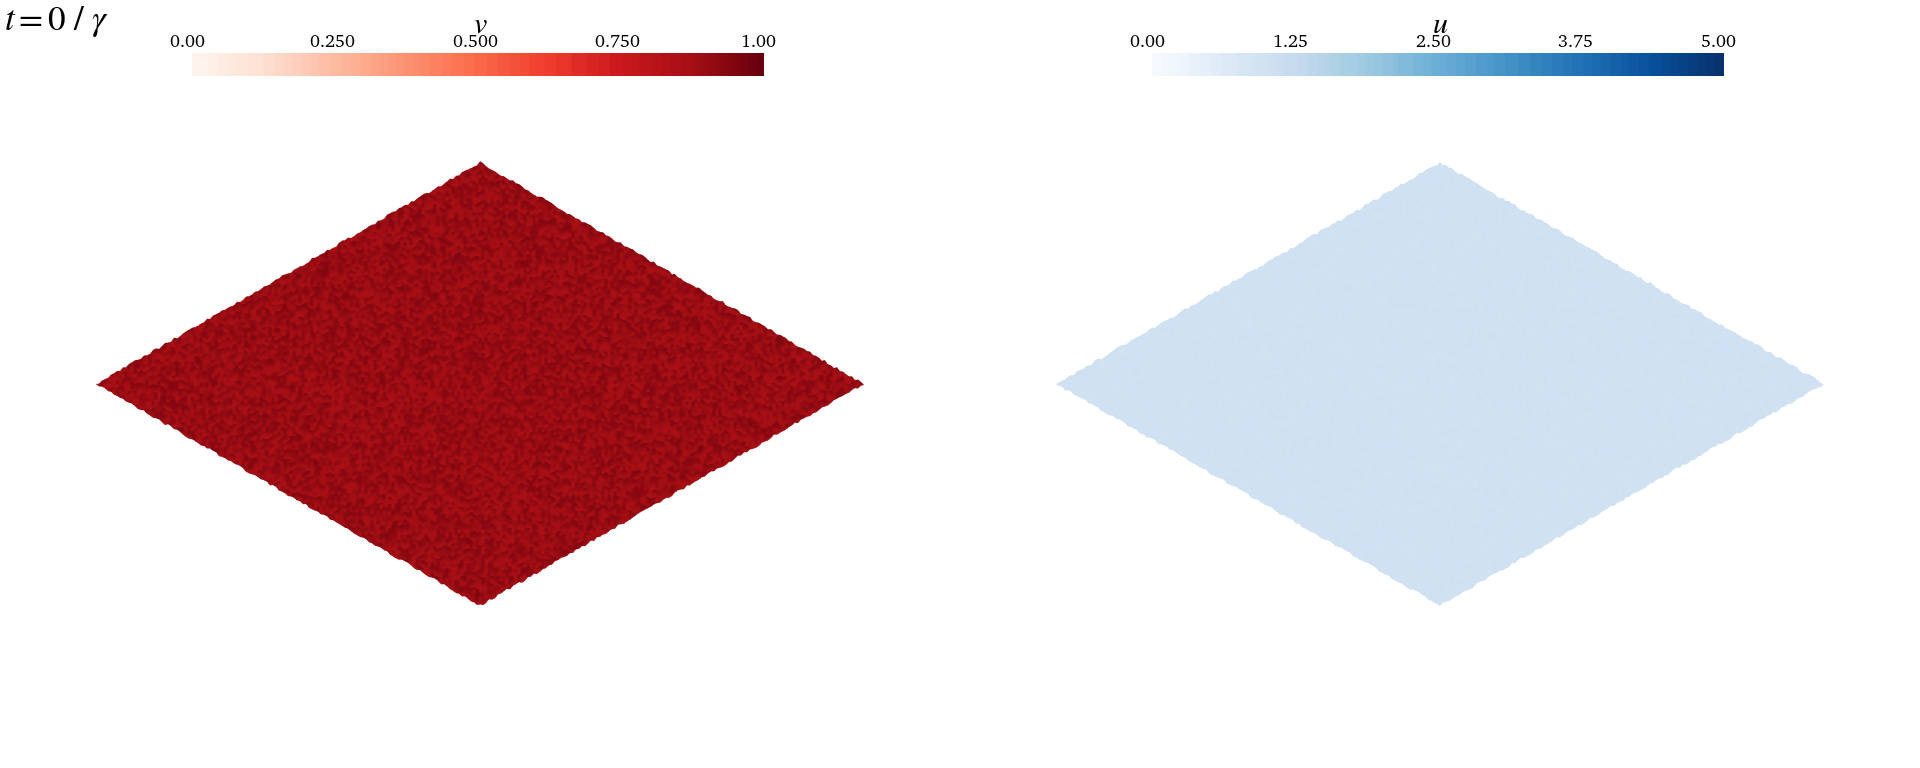
\includegraphics[width=\linewidth]{img/simulation_frames/schnakenberg_1.png}
        \caption{Caption 1}
    \end{subfigure}

    \vspace{0.4cm}

    \begin{subfigure}{\textwidth}
        \centering
        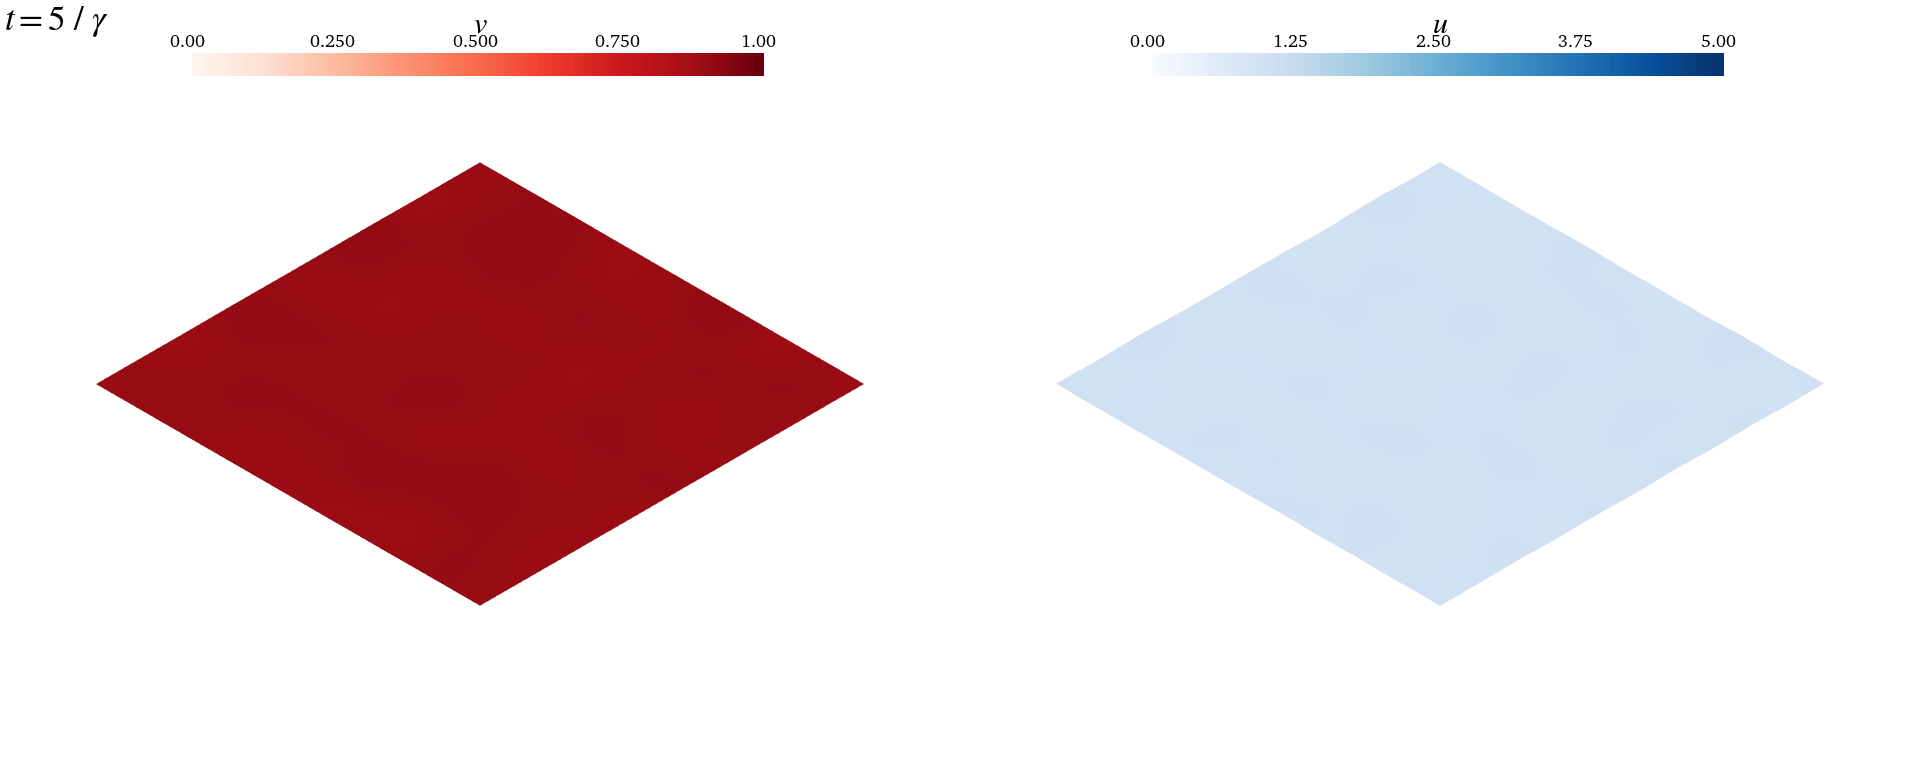
\includegraphics[width=\linewidth]{img/simulation_frames/schnakenberg_2.png}
        \caption{Caption 2}
    \end{subfigure}

    \vspace{0.4cm}

    \begin{subfigure}{\textwidth}
        \centering
        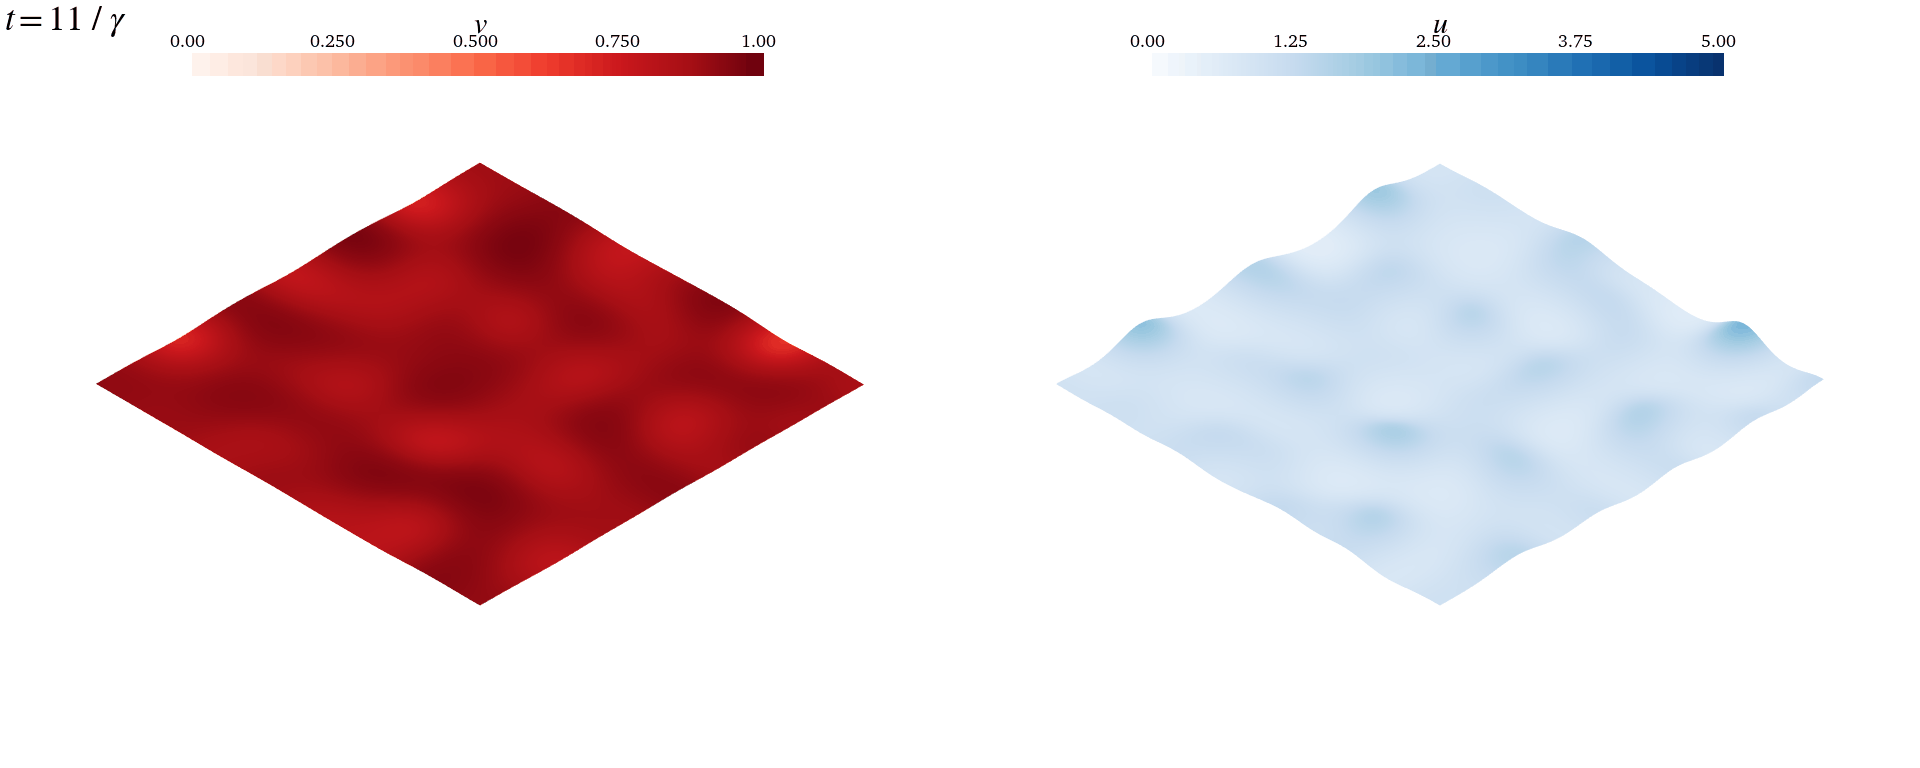
\includegraphics[width=\linewidth]{img/simulation_frames/schnakenberg_3.png}
        \caption{Caption 3}
    \end{subfigure}

    \caption{Overall figure caption.}
    \label{fig:schnakenberg_frames_1-3}
\end{figure}

\begin{figure}[htbp]
    \centering

    \begin{subfigure}{\textwidth}
        \centering
        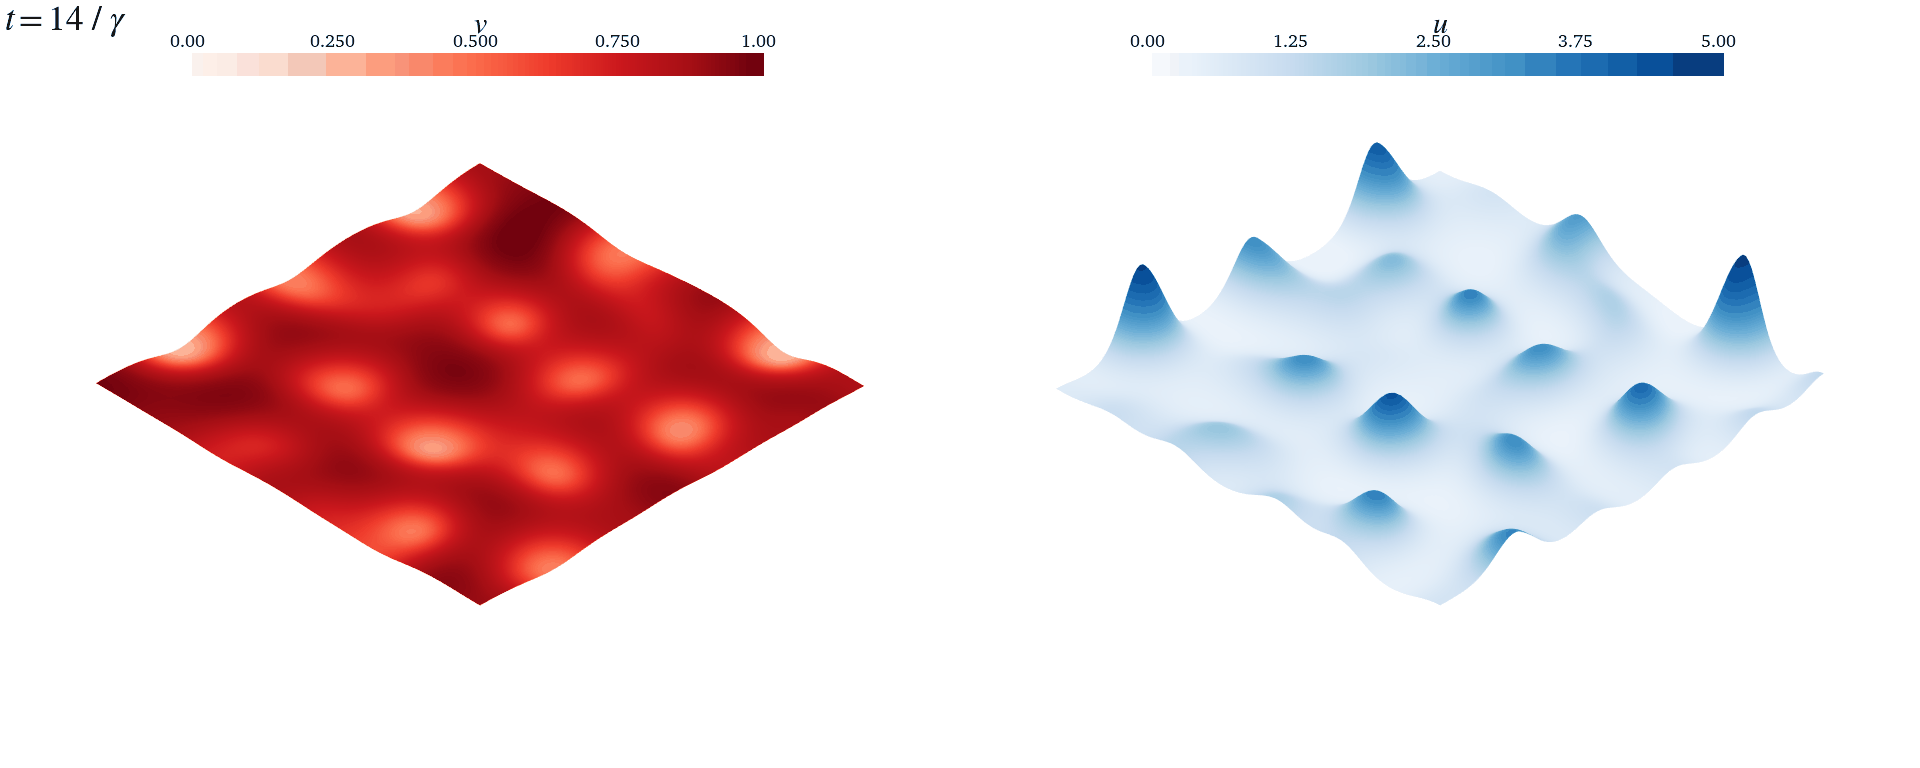
\includegraphics[width=\linewidth]{img/simulation_frames/schnakenberg_4.png}
        \caption{Caption 4}
    \end{subfigure}

    \vspace{0.4cm}

    \begin{subfigure}{\textwidth}
        \centering
        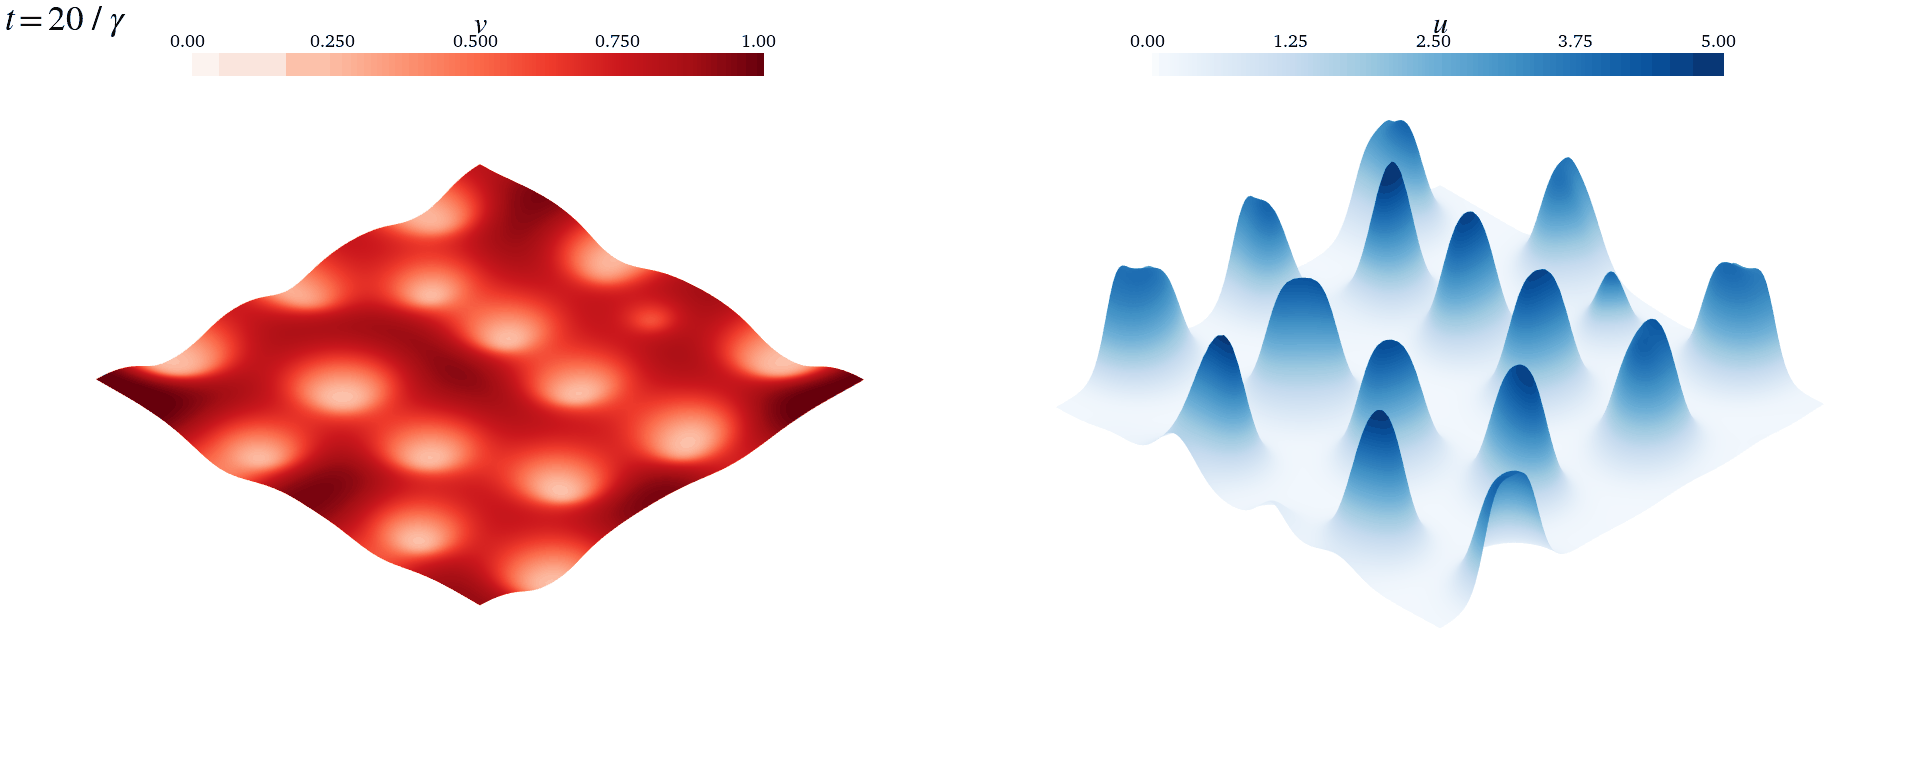
\includegraphics[width=\linewidth]{img/simulation_frames/schnakenberg_5.png}
        \caption{Caption 5}
    \end{subfigure}

    \vspace{0.4cm}

    \begin{subfigure}{\textwidth}
        \centering
        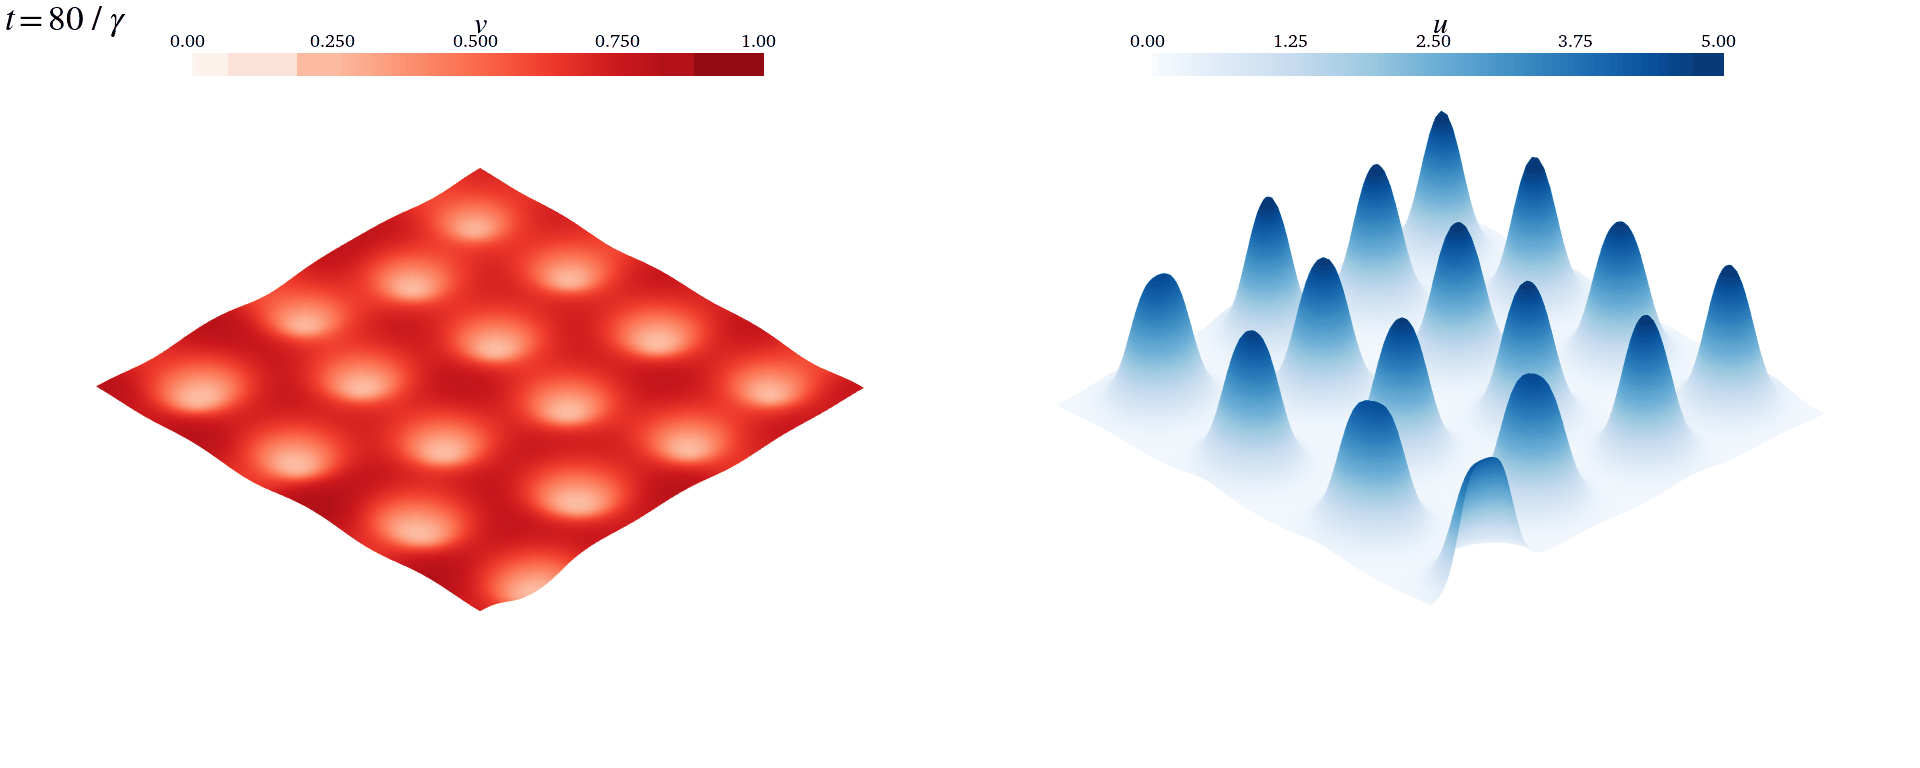
\includegraphics[width=\linewidth]{img/simulation_frames/schnakenberg_6.png}
        \caption{Caption 6}
    \end{subfigure}

    \caption{Overall figure caption.}
    \label{fig:schnakenberg_frames_4-6}
\end{figure}